\documentclass{article}

% if you need to pass options to natbib, use, e.g.:
%     \PassOptionsToPackage{numbers, compress}{natbib}
% before loading neurips_2021

% ready for submission
\usepackage[preprint]{neurips_2021}

% to compile a preprint version, e.g., for submission to arXiv, add add the
% [preprint] option:
%     \usepackage[preprint]{neurips_2021}

% to compile a camera-ready version, add the [final] option, e.g.:
%     \usepackage[final]{neurips_2021}

% to avoid loading the natbib package, add option nonatbib:
% \usepackage[nonatbib]{neurips_2021}
\usepackage[utf8]{inputenc} % allow utf-8 input
\usepackage[T1]{fontenc}    % use 8-bit T1 fonts
\usepackage[colorlinks = true, 
		    linkcolor = blue,
		    urlcolor  = blue,
            citecolor = blue,
            anchorcolor = blue]{hyperref}       
% hyperlinks
\usepackage{float}
\usepackage{url}            % simple URL typesetting
\usepackage{booktabs}       % professional-quality tables
\usepackage{amsfonts}       % blackboard math symbols
\usepackage{nicefrac}       % compact symbols for 1/2, etc.
\usepackage{microtype}      % microtypography
\usepackage{xcolor}         % colors
\usepackage{natbib}
\usepackage[pdftex]{graphicx}
\usepackage{siunitx} % Required for alignment
\sisetup{
  round-mode          = places, % Rounds numbers
  round-precision     = 2, % to 2 places
}
	
\bibliographystyle{unsrtnat}


\title{Extracting and evaluating educational concept dependencies from Large Language Models}

% The \author macro works with any number of authors. There are two commands
% used to separate the names and addresses of multiple authors: \And and \AND.
%
% Using \And between authors leaves it to LaTeX to determine where to break the
% lines. Using \AND forces a line break at that point. So, if LaTeX puts 3 of 4
% authors names on the first line, and the last on the second line, try using
% \AND instead of \And before the third author name.

\author{%
  Dominik Glandorf\\
  Matrikelnummer 6007407\\
  \texttt{dominik.glandorf@student.uni-tuebingen.de} \\
  \And
  Anastasiia Alekseeva\\
  Matrikelnummer 5994775\\
  \texttt{anastasiia.alekseeva@student.uni-tuebingen.de} \\
  \\
  GitHub repository: \url{https://github.com/mlcolab/learning-dependencies}
}

\begin{document}
\vspace*{-5mm}
\maketitle
\vspace*{-5mm}

\begin{abstract}
% What did we do?

% Why did we to it? What did we expect?

% How did we do it?

% What did we find out?

% What now?

\end{abstract}

\section{Introduction}
% Starting broad
% Field of contribution
Large Language Models (LLMs) are trained on immense corpora of text and have proven to build on embedded factual information when performing well in downstream tasks such as question answering. Accessing this knowledge, which is represented by billions of parameters and the network's architecture, has given rise to the research field of Knowledge Extraction from LLMs (\cite{cohen2023crawling}), which rests on the assumption that the language models can help retrieve information on the relation between entities. 

This work contributes to this field and aims to answer the question of whether LLMs generally are able to provide a valid dependency structure of educational concepts. To find the answer to the research question, we are going to solve two main subtasks: 1) extraction of implicit educational concept dependencies, and 2) evaluation of the retrieved dependencies or the resulting graphs by existing knowledge media.

Apart from the field of knowledge extraction from LLMs, which is a subfield of computational linguistics, our work may contribute to applied education sciences by improving computer-assisted education and creating new perspectives for a subfield of knowledge engineering that has rather stagnated in the previous years.

% What kind of information do we want to extract?
%% Problem of sequencing in Instructional Design:
In particular, effective and efficient instruction does not only incorporate what to teach but also how to teach, especially the order of instruction.  It is proven that \textit{instructional sequencing} enhances the process of learning when prerequisites of educational content are known to the student or taught first \citep{morrison2019designing}.
% Definition concepts
Within educational content, Merill (1983) differentiated facts, concepts, principles, rules, procedures, interpersonal skills, attitudes, and their sole recall from their application.
% TODO: explain this more:
We will focus on concepts and their relations defined understanding. 

% Concept dependency
% Assumption: information about dependencies between concepts makes instructional sequencing more effective in terms of learning

To be more precise, if one concept is a prerequisite of another, we refer to this relation as a concept dependency. For example, to understand the concept of a derivative, having knowledge about the concept of a function will facilitate or even enable learning. When the dependencies are thought of as directed edges between nodes that represent concepts, a concept dependency graph emerges which is a special type of a knowledge graph \citep{wang2016using}. This graph is also called \textit{concept map} in the field of Learning Sciences.
% TODO: provide a (graphical) example of a small concept map
% Why is is important?
The graph can be used to advance curriculum planning (\cite{yang2015concept}), especially for new topics that might not be covered in textbooks or automated assessment (Wang, 2015).

% What is the gap in research that we tackle?
% What is our research question?
% How to extract educational concept dependencies that are implicit and evaluate them using existing knowledge media?
%In this work, we tackled the question how to extract this particular knowledge graph and how to evaluate its quality in a scalable manner.

% What can we contribute?
% 1. No benchmark available -> we set up an evaluation framework based on textbooks and Wikipedia
To conclude, our main contributions are the following.
First, there is little research on how to evaluate the precision of extracted concept dependencies. Therefore, we propose a set of methods to use existing unstructured knowledge sources, namely Wikipedia and textbooks, to create baselines for evaluation. Due to the heuristic character of these methods, we conducted a manual assessment to test their suitability for our purpose. The resulting dataset can be used as a baseline for further research.

% 2. Emerging field of prompt engineering -> we engineered a simple but effective prompt process to query a LLM
Second, the emerging field of prompt engineering provides a constellation of commands to query LLMs, the majority of which are experimental and cannot be considered fully reliable. We propose a method called \textit{output refeeding} that allows mining the educational concept dependencies by sequentially querying the language generation model and transforming its answers into a knowledge graph.

\subsection{Related work}
% Field: Concept Dependency Extraction
% of interest: How are concept dependencies defined?
\cite{talukdar2012crowdsourced} defined the prerequisite relation in terms of the consumption of information about concepts. Vuong (2011) if a better graduation rate given prerequisite knowledge is fulfilled. Concepts are often equated with Wikipedia articles (Talukdar and Cohen, 2012; Wang, 2015).

% Other approaches: Learning Path Analysis and Expert Knowledge
Prerequisites can be inferred from learner behavior by testing their performance after being presented with different instructional sequences (Pavlik et al., 2008, Vuong et al., 2011). However, this has the disadvantage of disengaging users with too difficult concepts before teaching easier or necessary ones. Experts usually dispose of the required knowledge about concepts to create concept maps. The high cost of expert knowledge motivates the automated extraction of concept dependencies from appropriate sources.

% Field: Textbook Knowledge Extraction
% of interest: How are relationships betweens concepts extracted?

% Field: Prompt Engineering for Knowledge Graph creation
% of interest: How can we get internal representations out of a language model?
% Cohen, 2023 

Multiple approaches of prompt engineering for graph creation have been recently developed. Few-shot prompting proved successful (\cite{cohen2023crawling})

% GraphGPT

\section{Method}
% Section summary
In this section, we will first detail our research design and then the characteristics of our information sources as well as the methods that we used to produce the knowledge graph. 

\subsection{Research design} 
% two baseline methods: textbooks and Wikipedia
% information extraction: one LLM method
% evaluation
% 1. manual inspection via DashBoard
% 2. manual labeling
% 3. convergence between LLM and baselines
The choice of methodology reflects the fact that our research is located at the intersection of educational sciences and computational linguistics. On the one hand, we want to achieve a high performance of a state-of-the-art LLM in the downstream task of knowledge graph extraction. On the other hand, we consider a complex educational problem that cannot be purely simplified to classical machine learning metrics but requires additional qualitative assessment to ensure that our results can be educationally sound.

First of all, we restricted the concepts, of which dependencies we assessed, to the domain of linear algebra. This design choice was caused by the assumptions that the highly structured domain of mathematics provides enough relations to capture on the one hand and that linear algebra is a rather matured branch of mathematics were enough data exists for our baselines to be created as well as the LLM to have learned about from its own training data. Due to the use of linear algebra in different disciplines the potential value of results is also increased.

To be able to measure the LLM's performance, we had to come up with a target dataset. This dataset needs to describe a graph, containing the concepts as vertices and their dependencies as directed edges. Since no ground-truth, large-scale knowledge graph of concept dependencies was available to us and might even be impossible to achieve for our educational problem, we chose two sources of educational knowledge to serve as our knowledge base, namely textbooks, and Wikipedia. Due to their end-user-facing format, further processing of the input data (PDFs and webpages) was required to create the above-defined data structure. To make the graphs comparable with each other, the set of concepts was restricted to the union of all concepts indicated in all textbooks' indices. The LLM was prompted and the responses were also further processed to create the knowledge graph.

After creating the baseline datasets and the output to evaluate, we started qualitative evaluation using an interactive dashboard, that visualized the dependency structure. This step was done to get an impression of the general suitability of all three pipelines and identify potential reasons for performance losses. Then a subset of all three datasets was manually rated by multiple raters to not only infer their overall quality but also assess the human performance on the problem. We finally checked for outputs for convergence to give suggestions for a scalable, low-cost evaluation system of future (versions of) LLMs. The former evaluations are rather typical in educational research whereas the latter enables the creation of large-scale datasets, potentially suitable to train and fine-tune machine learning models.

\subsection{Baseline extraction}
This section details how we used Wikipedia and textbooks to set up the evaluation baselines for the LLM.

\subsubsection{Wikipedia}
% Why Wikipedia? 
The choice of the online encyclopedia Wikipedia as an educational information source is a result of its inherent graph structure induced by hyperlinks between articles and empirical evidence of its suitability for this purpose. %TODO: Add knowledge extraction literature from 2015/16
Especially, the platform is claimed to cover concepts up to the complexity of undergraduate curricula to a high extent, which aligns well with our chosen domain of linear algebra, which is usually taught to undergraduate students. The focus on dependencies required for understanding a concept makes an encyclopedia an ideal source because its articles are usually written to enable a fast understanding of the article's topic. In an online encyclopedia, hyperlinks provide additional information. In Wikipedia, each content article begins with a short summary, often serving as a definition and embedding the topic into its context, before in-depth information follows. In this summary text, we assume an implicit order from most important to least important concepts that are used to explain the topic without digressing to other concepts or unimportant information. The involved concepts are inferred to be a dependency. To prevent direct cycles by two concepts involving each other in their explanation, the one that refers earlier to the other is considered to be dependent on the latter. Situations, where the introduction of concept A states that concept B is dependent on it might be resolved like this.

Our assumptions about the Wikipedia structure were operationalized in the following way to compute the dependencies for a given concept. Every link in the first content paragraph containing a link is considered a candidate dependency. Therefore, any non-content paragraph such as advice regarding irrelevance or missing sources has to be removed beforehand. First, links to categories or fields such as "Mathematics" or "Linear Algebra" are removed based on a manually composed blacklist (a more sophisticated, automatic pruning could make use of Wikipedia's category pages). Then links to articles about persons are filtered out since these do not represent educational concepts. The same applies to links to pages that contain unexpected content such as disambiguation pages. Subsequently, cyclic dependencies are resolved as described above using both character positions of the symmetric links in the text. If more candidates remain than the threshold of 5, only the first 5 were kept, using the assumption of decreasing importance from the beginning on and the constraint of some sparsity of the resulting graph. This set of concepts is then taken as the concept's dependencies. 
%TODO: add amount of data

The described procedure was executed for every concept in the set resulting from the textbook baseline. Although Wikipedia theoretically offers a larger number of articles about the topic, we decided to stick with the limited set to maintain comparability. However, we decided against restricting the dependencies to other concepts in the set to also be able to evaluate the recall of the methods. The computational complexity of the procedure is relatively low and most time is spent on requesting Wikipedia web pages for the concepts and the links. The overall time was hence reduced by caching the responses to these requests. The technical implementation in Python required engineering our own Wikipedia API using the Python libraries requests and BeautifulSoap. The tools are used to download the page content and conveniently access elements such as links or special HTML tags indicating that an article is about a person.

\subsubsection{Textbooks}
% Why textbooks?
We chose student textbooks as the complementary information source besides the general purpose knowledge base Wikipedia because they are written by experts specifically for the purpose of educational knowledge transfer to learners. This not only leads to comprehensive coverage of carefully selected concepts that are considered relevant by the authors but also to a specific structure that we planned to exploit with our baseline extraction method, namely a pedagogic linearization of topics. More precisely, the authors are expected to first introduce concepts that more complex concepts build upon. Another useful structure in textbooks is the index, which provides a comprehensive list of concepts covered in the book and defined as its own entities.

% Amount of data
Due to the popularity of the topic of Linear Algebra, we could easily identify ten free textbooks on the topic and obtain their PDF representations (either directly typeset in this format or scanned and processed with OCR). The books comprised 584 pages on average (652,297 characters) and had a median of 382 index entries.

% Steps of processing
% preprocessing

% Wikisearch: query Wikipedia search engine for keyword (and field) and rank results based on Levenshtein distance
First, the textbooks were converted from PDF format to unformatted text. To identify all concepts of interest covered in a book, the pages containing the index were identified and each index entry with its corresponding pages was extracted in a semi-manual fashion. This required setting parameters such as the title, position of the columns and the type of nesting. To enable comparing the knowledge graph across the baselines, we decided to use the set of Wikipedia articles as the set of concepts, meaning that only a Wikipedia article title can serve as a vertex. This required mapping from each index entry to the closest Wikipedia article. For this disambiguation, the term was introduced into the Wikipedia search engine suffixed with the field term "(Mathematics)" to hint to the general area. Due to the high diversity of the resulting 10 articles, their names were string-matched with the search term (without the suffix) using the Levenshtein distance (provided by a Python library). The article title with the lowest distance that did not refer to an disambiguation page was the result of this so-called \textit{Wikisearch disambiguation}.

For the depdency extraction we came up with three distinct strategies. The first is solely based on indices whereas the latter also uses the full text. The first strategy is called order pruning and is interested in unlikely dependencies on the graph. It checks whether two concepts are introduced at least twice in a specific order and rules out the dependency that is not suggested by this order. For example if concept A is introduced twice before concept B, it is unlikely to depend on a concept introduced later by two independent authors. This strategy might work for a massive amount of books which was not available to us, but Wikifier \citep{brank2017annotating} was exploited for entity recognition and disambiguation.



% relation extraction

% entity recognition and disambigation
% Wikifier: identify entity mentions using link targets and PageRank
% common introductory usage: identify other concepts that are most often mentioned on the first page given in the index across all books
% order pruning:  identify unlikely dependencies based on a certain number of books that introduce concepts in a particular order

We used 10 books that are free and available online. 

\subsection{LLM extraction}
% description of T0PP and our infrastructure
% • Fine-tuned BLOOM on several question-answering datasets
% • 11 billion parameters (44GB RAM) • ~3-10 seconds per request on our infrastructure

% description of extraction procedure
% 1. output refeeding
% first prompt: {definition} := What is the mathematical definition of {concept}?
% second prompt:  {list of dependencies} := What mathematics concepts are mentioned here: {definition}
% 2. response parsing to Wikipedia article
% {canonical list of dependencies} :=Wikisearch disambiguation on {list of dependencies}

\begin{figure}
    \centering
    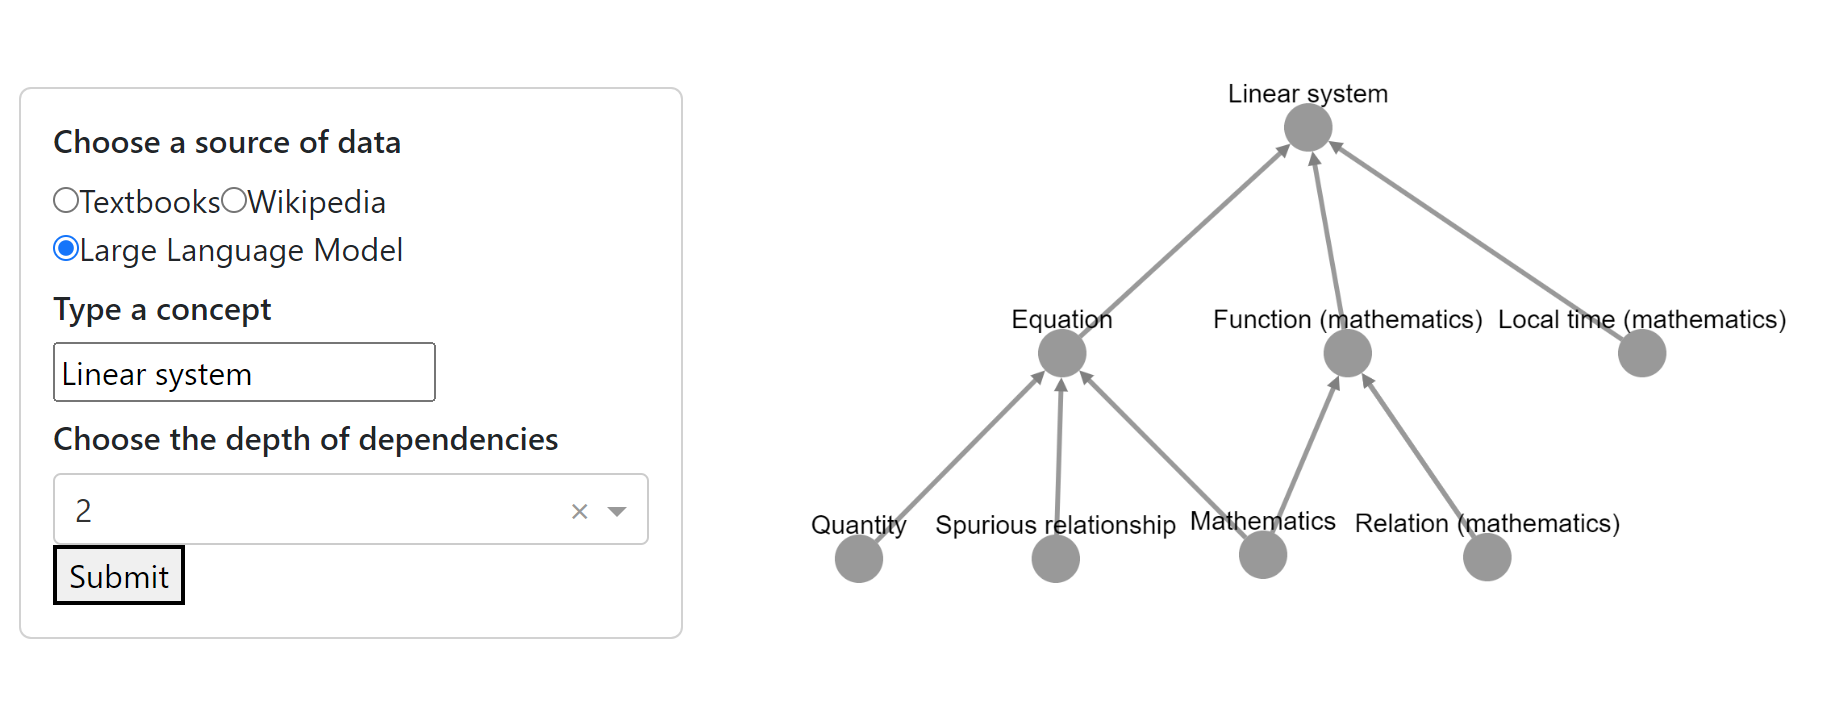
\includegraphics[width=.95\textwidth]{img/dash_example.png}
    \caption{A screenshot of the intercative application.}
    \label{fig:dash_example}
\end{figure}

\subsection{Manual inspection via Dashboard}
We developed a Dashboard via graphing library for Python Plotly\footnote{https://plotly.com/python/} (Fig.\ref{fig:dash_example}). The application is devised so that one could examine the resulting graph itself in a convenient environment. It allows plotting the concept dependencies graphs for three knowledge sources or types of dependency mining methods (LLM, Wikipedia, and textbooks) for different levels of dependencies.   



\subsection{Manual baseline}
% procedure to assess the accuracy of output

\subsection{Convergence statistics}
% for which concepts did we compare what to see what

\section{Results}
% Case Study using Dashboard

%Manual baseline
% Interrater reliability
% How good are the baselines?
% How good is the LLM?
% diagram


\begin{figure}[H]
    \centering
    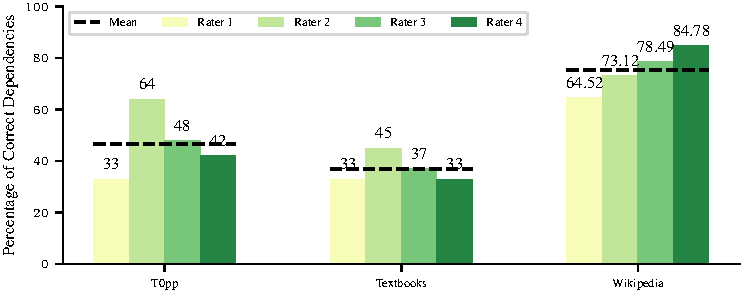
\includegraphics[width=.95\textwidth]{img/rating.pdf}
    \caption{Rating.}
    \label{fig:rating}
\end{figure}

\begin{figure}[H]
    \centering
    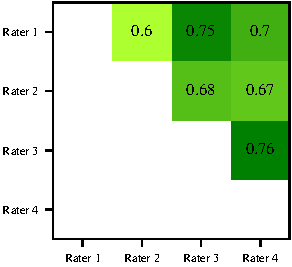
\includegraphics[width=.4\textwidth]{img/kappa.pdf}
    \caption{Interrater reliability, kappa coefficient.}
    \label{fig:kappa}
\end{figure}

%Convergence statistics
% diagram for similarity of outputs

\begin{figure}
    \centering
    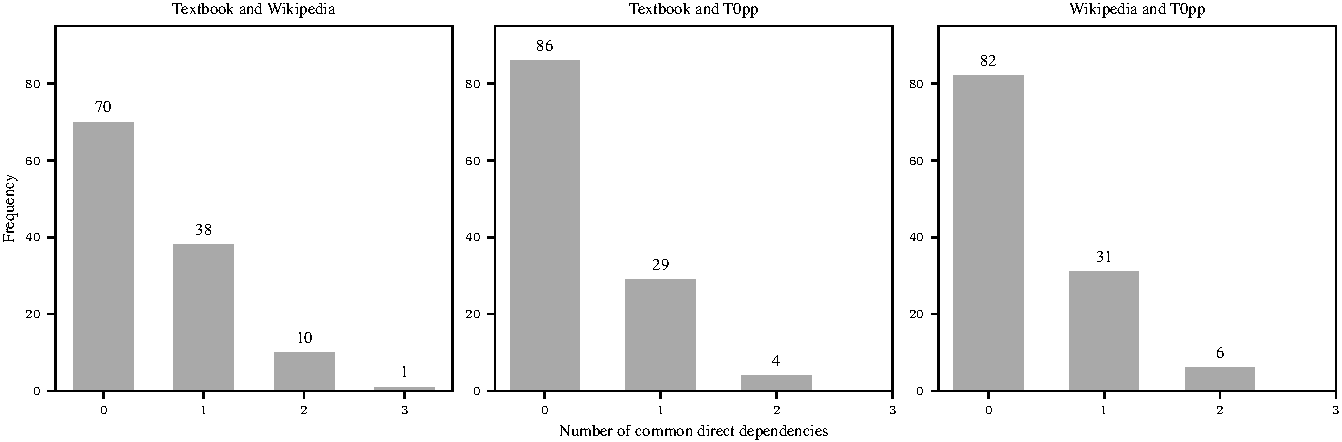
\includegraphics[width=.95\textwidth]{img/comp_direct_deps.pdf}
    \caption{Convergence metrics. Number of common direct dependencies between sources.}
    \label{fig:comp_direct_deps}
\end{figure}

\section{Discussion}
% What is our main result?
% we are able to make the implicit knowledge explicit far above chance level
% problem is very complex -> humans do not fully agree
% Wikipedia might be the best source to automatically evaluate the output

% What are potential flaws?

% disambiguation already includes noise
% error propagation

% we only evaluated up to two levels of the graph, not the graph as a whole. different level of abstractions in extracted dependencies
% (in)direct cycles
% is there even something like a gold standard? some educational reflection about different didactic approaches and more depth than just understanding the definition of a topic
% Cohen et al (2023) think that there is no gold standard, ground truth.

Each information extraction method is not fully independent of the other, in particular, entity recognition and concept disambiguation steps in the procedure for LLM and textbooks depend on Wikipedia.

% we are still using the language generator, so it is just another downstream task, maybe it is more of a philosophical question what is implicit/explicit knowledge


% + "I don't know" option in the prompt engineering part
% + Google search

% Q: Outlook and Future research ideas:

As shown, current LLMs are not sufficiently precise in creating concept maps, which confirms previous research \cite{hwang2021comet}. This could be improved by training the pre-trained models on the knowledge graph data mined from Wikipedia or any other reliable sources of concept dependencies in a specific subject of instruction \cite{west2022symbolic}.
% advancements in LLMs that are interesting for us
% use cases in education



\bibliography{references.bib}

\newpage


\section{Appendix}



\begin{figure}[H]
    \centering
    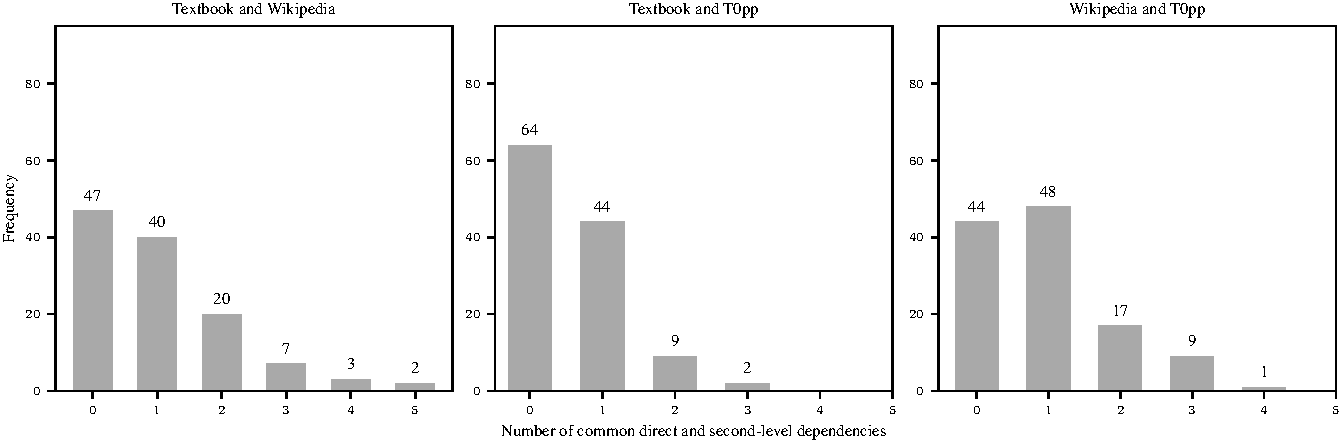
\includegraphics[width=.95\textwidth]{img/comp_second_deps.pdf}
    \caption{Convergence metrics. Number of common direct and second-level dependencies between sources.}
    \label{fig:comp_second_deps}
\end{figure}






\end{document}
